\begin{center}
    \(
    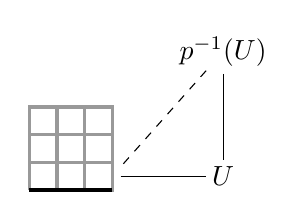
\begin{tikzpicture}[x=1em, y=1em, baseline=1em]
        \draw[very thick, black!40]
            (0,0)--(3,0)--(3,3)--(0,3)--(0,0)
            (1,0)--(1,3) (2,0)--(2,3)
            (0,1)--(3,1) (0,2)--(3,2);
        \draw[very thick] (0,0)--(3,0);
        \draw[-{\tip}, shorten <= 3pt, shorten >= 6pt] (3,.5)--(7,.5);
        \draw[-{\tip}, shorten <= 8pt, shorten >= 6pt] (7,5)--(7,.5);
        \draw[-{\tip}, shorten <= 6pt, shorten >= 8pt, dashed] (3,.5)--(7,5);
        \filldraw 
            (7,0.5) node{$U$}
            (7,5) node{$p^{-1}(U)$};
    \end{tikzpicture}
    \quad\leadsto\quad
    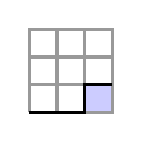
\begin{tikzpicture}[x=1em, y=1em, baseline=1em]
        \fill[blue!20] (2,0)--(2,1)--(3,1)--(3,0);
        \draw[very thick, black!40]
            (0,0)--(3,0)--(3,3)--(0,3)--(0,0)
            (1,0)--(1,3) (2,0)--(2,3)
            (0,1)--(3,1) (0,2)--(3,2);
        \draw[very thick] (0,0)--(2,0)--(2,1)--(3,1);
    \end{tikzpicture}
    \quad\leadsto\cdots\leadsto\quad
    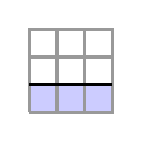
\begin{tikzpicture}[x=1em, y=1em, baseline=1em]
        \fill[blue!20] (0,0)--(0,1)--(3,1)--(3,0);
        \draw[very thick, black!40]
            (0,0)--(3,0)--(3,3)--(0,3)--(0,0)
            (1,0)--(1,3) (2,0)--(2,3)
            (0,1)--(3,1) (0,2)--(3,2);
        \draw[very thick] (0,1)--(3,1);
    \end{tikzpicture}
    \quad\leadsto\cdots\leadsto\quad
    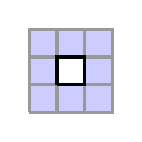
\begin{tikzpicture}[x=1em, y=1em, baseline=1em]
        \fill[blue!20] (0,0)--(0,3)--(3,3)--(3,0);
        \draw[very thick, black!40]
            (0,0)--(3,0)--(3,3)--(0,3)--(0,0)
            (1,0)--(1,3) (2,0)--(2,3)
            (0,1)--(3,1) (0,2)--(3,2);
        \filldraw[very thick, fill=white] (1,1)--(2,1)--(2,2)--(1,2)--(1,1);
    \end{tikzpicture}
    \quad\leadsto \Attention
    \)
\end{center}